\paragraph{QuizziPedia::Front-End::ModelViews::TrueFalseQuestionsModelView}
\begin{figure} [ht]
	\centering
	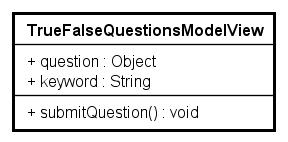
\includegraphics[scale=0.80]{UML/Classi/Front-End/QuizziPedia_Front-end_ModelView_TrueFalseQuestionsModelView.png}
	\caption{QuizziPedia::Front-End::ModelViews::TrueFalseQuestionsModelView}
\end{figure} \FloatBarrier
\begin{itemize}
	\item \textbf{Descrizione}: classe di tipo modelview la cui istanziazione è contenuta all'interno della variabile di ambiente \$scope di \textit{Angular.js\ped{G}}. All'interno di essa sono presenti le variabili e i metodi necessari per il \textit{Two-Way Data-Binding\ped{G}} tra la view \texttt{TrueFalseQuestionsView} e il controller \texttt{TrueFalseQuestionsController}; 
	\item \textbf{Utilizzo}: viene utilizzata per effettuare il \textit{Two-Way Data-Binding\ped{G}} tra la view \texttt{TrueFalseQuestionsView} e il controller \texttt{TrueFalseQuestionsController} rendendo disponibili variabili e metodi;
	\item \textbf{Relazioni con altre classi}:
	\begin{itemize}
		\item \textit{IN} \texttt{TrueFalseQuestionsController}: questa classe permette di gestire la creazione e la modifica di una domanda vero/falso;
		\item \textit{OUT} \texttt{TrueFalseQuestionsView}: view contenente le direttive per creare una domanda vero/falso.
	\end{itemize}
	\item \textbf{Attributi}:
	\begin{itemize}
	  \item \texttt{+ question: Object} \\ Oggetto contenete i dati della domanda, ovvero:
	  \begin{itemize}
		\item \texttt{questionText: String}: identifica il testo della domanda;
		\item \texttt{image: String}: identifica l'url di una possibile immagine nella domanda;
		\item \texttt{answers: Array}: array che contiene coppie di valori. Queste coppie sono formate da:
		\begin{itemize}
			\item \texttt{type: String}: indica la tipologia della risposta;
			\item \texttt{text: String}: contiene il testo dell'affermazione;
			\item \texttt{url: String}: rappresenta l'immagine della risposta;
			\item \texttt{attributesForTForMultiple: Mixed}: contiene i seguenti attributi:
			\begin{enumerate}
				\item \texttt{isItRight: Boolean}: contiene se la risposta è vera o falsa.
			\end{enumerate}
		\end{itemize}
		\item \texttt{+ keyword: String} \\ Attributo contenente la keyword associata alla domanda/questionario;
	\end{itemize}
	\end{itemize}
	\item \textbf{Metodi}:
	\begin{itemize}
		\item \texttt{+} \texttt{submitQuestion(): void}\\ 
		Metodo che gestisce l’evento click sul pulsante di conferma sulla domanda. Raccoglie i dati dal modelview e li manda al server attraverso \texttt{QuestionService}. Poi verrà effettuato il redirect alla pagina di gestione delle domande oppure al questionario che si stava creando;
	\end{itemize}
\end{itemize}

